\documentclass[../TDT6.tex]{subfiles}%

\begin{document}
\section{Cycle de \textsc{Rankine}}
\enonce{%
Un moteur fonctionne avec une masse $m$ d'eau. Cette masse d'eau subit les
transformations suivantes~:
\begin{itemize}
	\item AB~: isotherme (A liquide saturant à $T_1$ et $P_1$~; B à $P_2$)~;
	\item BC~: échauffement réversible isobare qui amène l'eau à la température
	      $T_2$ (C liquide saturant)~;
	\item CD~: vaporisation totale sous la pression $P_2$ et à la température
	      $T_2$~;
	\item DE~: détente adiabatique réversible jusqu'à la température $T_1$~;
	\item EA~: liquéfaction totale à la température $T_1$.
\end{itemize}
La capacité thermique massique de l'eau liquide vaut $c_{\rm liq} =
	\SI{4.18}{kJ.K^{-1}.kg^{-1}}$. Dans le tableau suivant, on donne les
caractéristiques des points se trouvant sur la courbe de saturation aux pressions
$P_1$ et $P_2$.
\begin{table}[h!]
	\label{tab:rankine}
	\begin{center}
		\begin{tabular}{
				c
				S[table-format=1.3]
				S[table-format=3.2]
				S[table-format=1.2e1]
				S[table-format=1.3]
				S[table-format=3.2]
				S[table-format=4.1]}
			\toprule
			                                &
			{$P$ (\si{bar})}                &
			{$T$ (\si{K})}                  &
			{$v_{\ell}$ (\si{m^3.kg^{-1}})} &
			{$v_g$ (\si{m^3.kg^{-1}})}      &
			{$h_{\ell}$ (\si{kJ.kg^{-1}})}  &
			{$h_g$ (\si{kJ.kg^{-1}})}

			\\\midrule
			{$P_1$}                         &
			0.250                           & 338.15 & 1.02e-3 & 6.202 & 272.02 & 2618.4
			\\
			{$P_2$}                         &
			1.208                           & 378.15 & 1.05e-3 & 1.419 & 440.17 & 2683.7
			\\
			\bottomrule
		\end{tabular}
	\end{center}
\end{table}

\vspace{-20pt}
\begin{isd}
	La variation d'entropie massique d'un liquide pour une transformation d'une
	température $T_A$ à une température $T_B$ s'exprime
	\[
		\Delta{s}\ind{AB} = s \ind{B} - s \ind{A} = c\ind{liq}\ln \left(
		\frac{T\ind{B}}{T\ind{A}} \right)
	\]
	\tcblower
	La variation d'entropie massique lors d'un changement d'état est~:
	\[
		\Delta{s} = \frac{\Delta{h}}{T}
	\]
	avec $\Delta{h}$ la variation d'enthalpie massique lors du changement d'état et
	$T$ la température du changement d'état.
\end{isd}
\vspace{-15pt}
}%

\QR{%
	Tracer l'allure de deux isothermes d'\textsc{Andrews} dans le diagramme
	de \textsc{Clapeyron}. On fera apparaître la courbe de saturation. Dessiner
	l'allure du cycle sur ce même diagramme.
}{%
	\sswitch{
		\hfill
		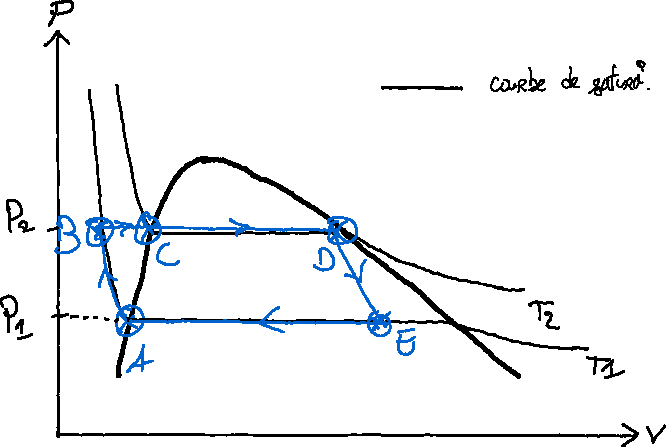
\includegraphics[width=.6\linewidth, valign=t]{rankine_cycle_A}
		\hspace*{\fill}
	}{
		\leavevmode\vspace*{-15pt}\relax
		\begin{center}
			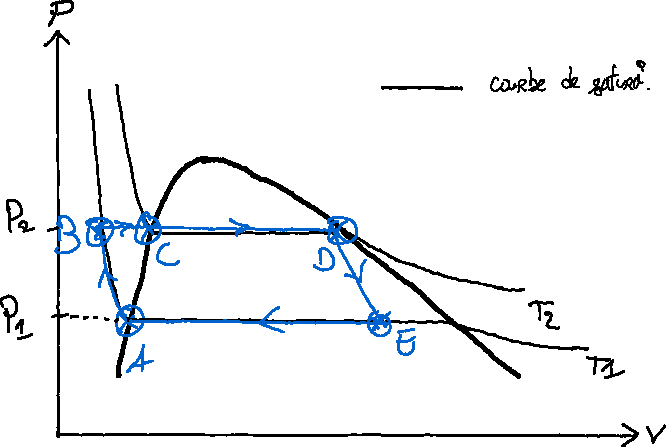
\includegraphics[width=.6\linewidth]{rankine_cycle_A}
		\end{center}
	}
}%

\begin{blocQR}
	\item
	\QR{%
		Montrer que la variation $s\ind{B} - s\ind{A}$ est nulle.
	}{%
		Pour un liquide,
		\begin{DispWithArrows*}
			\Delta{s}\ind{AB} &= c\ind{liq} \ln (\frac{T\ind{B}}{T\ind{A}})
			\Arrow{AB isoT\\$\Ra T\ind{B} = T\ind{A}$}
			\\\Lra
			\Aboxed{\Delta{s}\ind{AB} &= 0}
		\end{DispWithArrows*}
	}%

	\QR{%
		Exprimer $s\ind{C} - s\ind{B}$ en fonction de $c_{\rm liq}$, $T_1$ et $T_2$.
	}{%
		\begin{gather*}
			\Delta{s}\ind{BC} =
			s \ind{C} - s \ind{B} =
			c\ind{liq} \ln (\frac{T\ind{C}}{T\ind{B}})
			\Lra
			\boxed{s \ind{C} - s \ind{B} = c\ind{liq} \ln (\frac{T_2}{T_1})}
		\end{gather*}
	}%

	\QR{%
		Exprimer $s\ind{D} - s\ind{C}$ en fonction de $h_g(T_2)$, $h_{\ell}(T_2)$ et $T_2$.
	}{%
		CD est une vaporisation totale, il y a donc transition de phase~:
		\begin{gather*}
			\Delta{s}\ind{CD} = s \ind{D} - s \ind{C} = \frac{\Delta{h}\ind{CD}}{T_2}
			\\\Lra
			\boxed{s \ind{D} - s \ind{C} = \frac{h_g (T_2) - h_{\ell}(T_2)}{T_2}}
		\end{gather*}
	}%

	\QR<[ref=2) \alph* --]>{\label{q:2D}%
		Calculer $s\ind{E} - s\ind{D}$.
	}{%
		DE est adiabatique, soit $Q = 0 \Ra S\ind{ech,DE} = 0$ et réversible, soit
		$S\ind{cr,DE} = 0$~: elle est donc \textbf{isentropique}, c'est-à-dire
		\begin{gather*}
			\Delta{s}\ind{DE}\boxed{s \ind{E} - s \ind{D} = 0}
		\end{gather*}
	}%
\end{blocQR}

\QR{%
	Énoncer le théorème des moments.
}{%
	Sur un diagramme $(P,v)$ de transition de phase liquide-vapeur, les titres
	massiques $x_g$ et $x_{\ell}$ en gaz et liquide d'un équilibre diphasé se
	calculent par
	\[
		\boxed{x_g = \frac{\rm MG}{\rm LG}}
		\qet
		\boxed{x_{\ell} = \frac{\rm LM}{\rm LG}}
	\]
	avec M le point étudié de l'équilibre, L le liquide saturant correspondant et
	B la vapeur saturante correspondante.
}%

\QR{%
	Soit $x$ la fraction massique de vapeur en E. On admet que l'on peut
	appliquer le théorème des moments pour l'entropie. Déterminer $x$
	littéralement puis numériquement.
}{%
	\noindent
	\begin{minipage}[t]{.49\linewidth}
		Pour appliquer le théorème des moments, on prend E le point équivalent à M,
		A est équivalent à L et F le point équivalent à G. On a donc $\DS x =
			\frac{\rm AE}{\rm AF}$.
		\smallbreak
		Ainsi, $\DS x = \frac{s \ind{E} - s \ind{A}}{s \ind{F} - s \ind{A}}$. Or, on
		sait d'après~\ref{q:2D} que $s \ind{E} = s \ind{D}$, donc on peut réécrire
		\begin{gather*}
			s \ind{E} - s \ind{A} =
			s \ind{D} - s \ind{A} =
			\underbracket[1pt]{s \ind{D} - s \ind{C}}_{\frac{h_g (T_2) - h_{\ell}(T_2)}{T_2}} +
			\underbracket[1pt]{s \ind{C} - s \ind{B}}_{c\ind{liq} \ln (\frac{T_2}{T_1})} +
			\underbracket[1pt]{s \ind{B} - s \ind{A}}_{0}
			\\\Lra
			\Delta{s}\ind{AE} =
			\frac{h_g (T_2) - h_{\ell}(T_2)}{T_2} +
			c\ind{liq} \ln (\frac{T_2}{T_1}) + 0
		\end{gather*}
	\end{minipage}
	\hfill
	\noindent
	\begin{minipage}[t]{.49\linewidth}
		\vspace{0pt}
		\begin{center}
			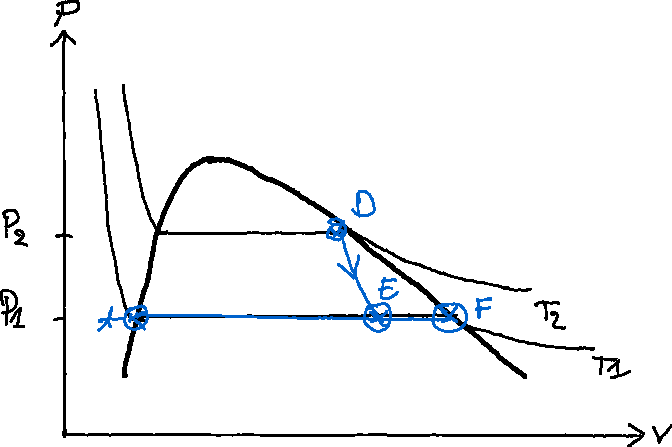
\includegraphics[width=\linewidth]{rankine_cycle_B}
		\end{center}
	\end{minipage}
	On ne connaît pas \textit{a priori} $s \ind{F} - s \ind{A}$. Cependant, cette
	transformation correspondrait à une transition de phase complète de vapeur
	saturante à $(T_1,P_1)$ en liquide saturant à $(T_1,P_1)$, dont on connaît la
	variation d'enthalpie~: $\Delta{h}\ind{AF} = h_g (T_1) - h_{\ell}(T_1)$. On
	connaît donc la variation d'entropie~:
	\begin{align*}
		\Delta{s}\ind{AF} = s \ind{F} - s \ind{A} & = \frac{h_g (T_1) - h_{\ell}(T_1)}{T_1}
		\\\Lra
		\Aboxed{
		x                                         & =
			\frac{T_1}{T_2} \frac{h_g (T_2) - h_{\ell}(T_2)}
			{h_g (T_1) - h_{\ell}(T_1)} +
			T_1 \frac{c\ind{liq} \ln (\frac{T_2}{T_1})}{h_g (T_1) - h_{\ell}(T_1)}
		}
		\\
		\text{avec}                               &
		\left\{
		\begin{array}{rclcrclcrcl}
			T_1           & =         & \SI{338.15}{K}
			              & \qMath{;} &
			h_g (T_1)     & =         & \SI{2.6184e3}{J.kg^{-1}}
			              & \qMath{;} &
			h_{\ell}(T_1) & =         & \SI{272.02e3}{J.kg^{-1}}
			\\
			T_2           & =         & \SI{378.15}{K}
			              & \qMath{;} &
			h_g (T_2)     & =         & \SI{2.6834e6}{J.kg^{-1}}
			              & \qMath{;} &
			h_{\ell}(T_2) & =         & \SI{4.4017e5}{J.kg^{-1}}
		\end{array}
		\right.                                                                             \\
		\makebox[0pt][l]{$\phantom{\AN}\xul{\phantom{x = \num{0.922}}}$}
		\AN
		x                                         & = \num{0.922}
	\end{align*}
	Il y a donc \SI{92.2}{\%} de vapeur. On remonte ainsi à $v\ind{E}$ par le
	théorème des moments~:
	\begin{align*}
		x        & = \frac{v\ind{E} - v_{\ell}}{v_g - v_{\ell}}
		\\\Lra
		\Aboxed{
		v\ind{E} & = v_{\ell} + x (v_g - v_{\ell})
		}
		\\
		\makebox[0pt][l]{$\phantom{\AN}\xul{\phantom{v\ind{E} = \SI{5.72}{m^3.kg^{-1}}}}$}
		\AN
		v\ind{E} & = \SI{5.72}{m^3.kg^{-1}}
	\end{align*}
}%

\QR{%
	Calculer les transferts thermiques massiques échangés lors des
	transformations BCD et EA.
}{%
	Entre B et C, la transformation est isobare donc
	\begin{DispWithArrows*}
		\Delta{H}\ind{BC} &= Q\ind{BC}
		\\\Lra
		\Delta{H}\ind{BC} &= mc\ind{liq}(T_2-T_1)
		\CArrow{$\mdiv m$}
		\\\Lra
		q\ind{BC} &= c \ind{liq}(T_2-T_1)
	\end{DispWithArrows*}
	Entre C et D, on a aussi une transformation isobare, donc
	\begin{DispWithArrows*}
		\Delta{h}\ind{CD} &= q\ind{CD}
		\\\Lra
		h_g (T_2) - h_{\ell}(T_2) &= q\ind{CD}
		\Arrow{On somme}
		\\\Lra
		\Aboxed{
			q\ind{BCD} &-
			c\ind{liq}(T_2-T_1) + \underbracket[1pt]{h_g (T_2) -
				h_{\ell}(T_2)}_{\Delta{h\ind{vap}(T_2)}}
		}
		\\
		\AN
		\makebox[0pt][l]{$\xul{\phantom{q\ind{BCD} = \SI{2.41}{MJ}}}$}
		q\ind{BCD} &= \SI{2.41}{MJ}
	\end{DispWithArrows*}
	Entre E et A,
	\begin{DispWithArrows*}[]
		\Delta{h}\ind{EA} = q\ind{EA} &= h\ind{A} - h\ind{E}
		\Arrow{$h\ind{A} = h_{\ell}(T_1)$\\$h\ind{E} = x h_g (T_1) +
			(1-x)h_{\ell}(T_2)$}
		\\\Lra
		\Aboxed{
			q\ind{EA} &=
			x \underbracket[1pt]{(h_{\ell}(T_1) - h_g (T_1))}_{\Delta{h}\ind{liq}(T_1)}
		}
		\\
		\AN
		\makebox[0pt][l]{$\xul{\phantom{q\ind{EA} = \SI{-2.16}{MJ}}}$}
		q\ind{EA} &= \SI{-2.16}{MJ}
	\end{DispWithArrows*}
	\begin{tcn}(rema)<lftt>{Remarque}
		On \textbf{reçoit} bien de la chaleur lors de la vaporisation, on en
		\textbf{cède} lors de la liquéfaction.
	\end{tcn}
}%

\QR{%
	Déterminer le rendement du cycle. Application numérique.
}
	\end{DispWithArrows*}
}%

\end{document}
